\documentclass{article}
\usepackage[utf8]{inputenc}
\usepackage{graphicx}
\usepackage{physics}
\usepackage[affil-it]{authblk} 
\usepackage{etoolbox}
\usepackage{lmodern}

\makeatletter
\patchcmd{\@maketitle}{\LARGE \@title}{\fontsize{16}{19.2}\selectfont\@title}{}{}
\makeatother

\renewcommand\Authfont{\fontsize{12}{14.4}\selectfont}
\renewcommand\Affilfont{\fontsize{9}{10.8}\itshape}

\title{CS 440 Project 1: A * is Born}
\author{Geet Purohit 188001760 and Miguel Ranjo 188002839}
\affil{Fast Trajectory Replanning}

\date{October 22, 2021}

\begin{document}

\maketitle

\section*{Introduction}

For this project, we built a program to traverse from point A to point B using A* algorithm. Python was used to build the project and mazes were built randomly to prove the efficacy of our implementation.

\section*{Part 0}

Our first job was to create $50$ mazes of size $101$ x $101$.  We begin by generating a numpy zero array. From there we begin at a random point of the graph and make it unblocked. From there we start generating paths. We visit random neighbors using random first depth search algorithm making sure to record all points to ensure we visited all points. Each time we look at a point, a uniform random number is generated between $0$ and $1$. If that number is $<.3$, the cell is blocked and otherwise, it is kept unblocked.

It is possible for a cell to have all its neighbors visited (considered a dead end). From here, we pop that cell from the stack and continue until we reach a cell with unvisited neighbors. We continue calculating random numbers from there. We also have a supplementary two dimensional array that records whether a cell has been visited and this can be used to ensure that we perform the above random number method on each cell.
\newpage
A sample of a maze seen through our visualizer is demonstrated below:


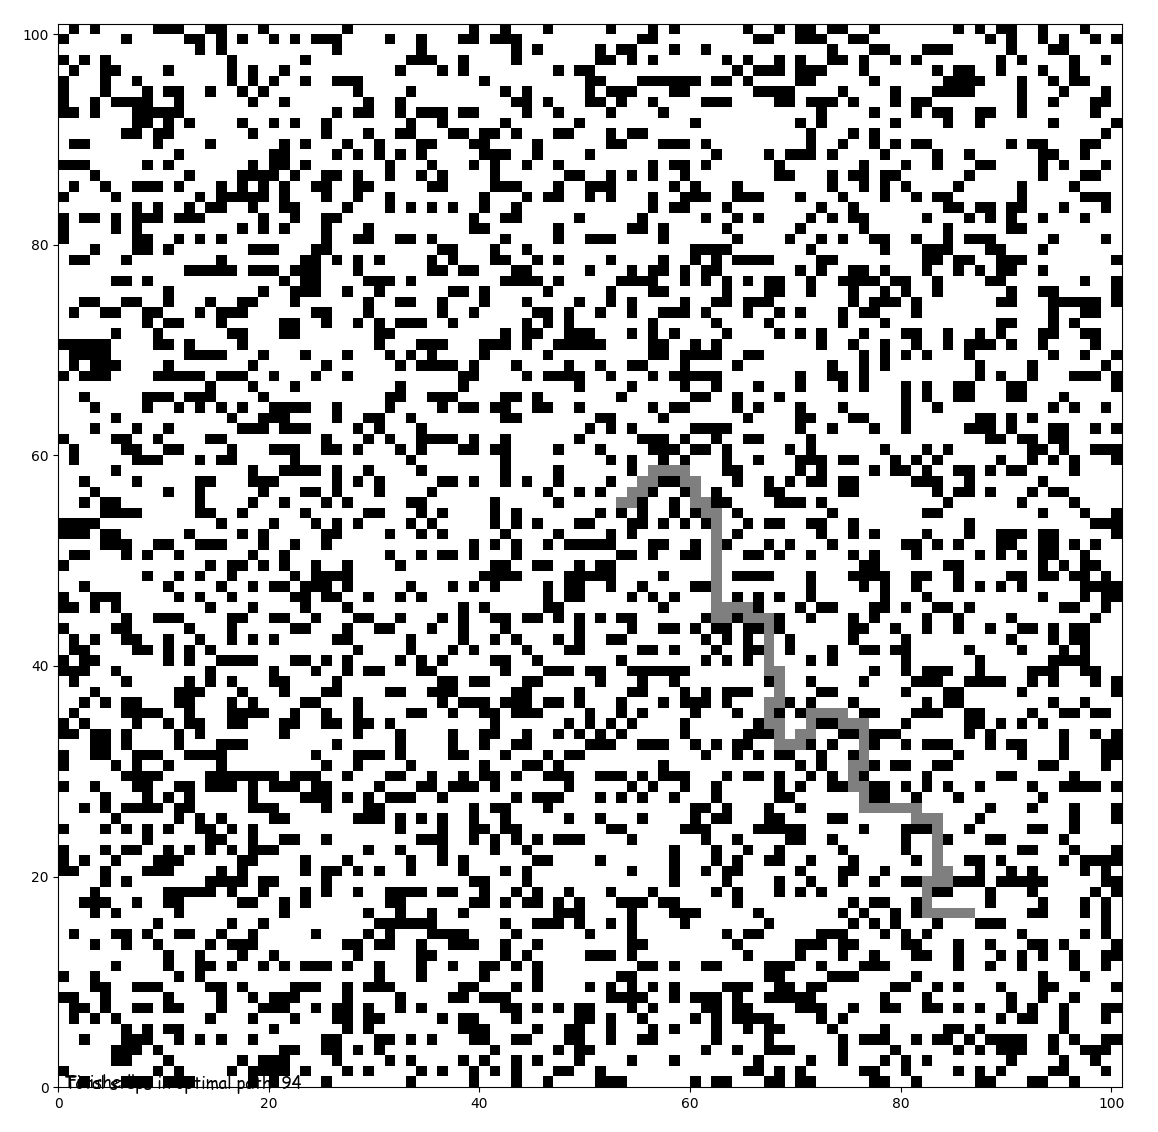
\includegraphics[scale=.3]{Figure_1.png}


\section*{Part 1}

a. In this question, our program is finding a path from E2 to E5. We can easily eliminate going South as it is an invalid choice. Considering that we are trying to find the shortest possible path, the agent will move assuming that no cells are blocked. The target is directly East, so moving North or West is counterproductive to its goal. Hence it will move East, the most direct path to the target.\\
\\
b. We can easily prove this as the number of cells is finite, so the agent is bound to exhaust all option in reaching its goal or reach it. In its worst case, the agent traverses the entire map. Due to A* having a list of previously visited points, the agent will never move to previously traversed cells. Hence there will be no infinite looping as it traverses the entire map. If the path is blocked, the agent will see this when it has traversed ever cell it could and did not reach its goal. At this point, the program will stop executing. To sum it up, the number of moves is bounded from above by the number of unblocked cells squared. We can further prove this as the number of moves the agent can make whenever it performs an A* iteration is at most the total number of cells. Hence the moves must be less than or equal to the number of cells. A* is called repeatedly and it must be at most equal to the number of cells. With this we have our total moves which must be bounded from above.




\section*{Part 2}

A* With Smaller G (Average of $50$ runs)

Total Time Step: $135.565$

Actual Cost: $107.652$

Number of A Star Iterations: $28.913$

Time Cost: $0.926$ seconds

Number of Expanded Cells: $15209.296$

Costs for optimal path: $107.652$
\\ 
\\A* With Bigger G (Average of $50$ runs)

Total Time Step: $179.833$

Actual Cost: $142.771$

Number of A Star Iterations: $38.0625$

Time Cost: $0.0964$ seconds

Number of Expanded Cells: $1718.375$

Costs for optimal path: $142.771$
\\
\\After coding both versions, we found it efficient to break ties in favor of higher g-values instead of lower ones. This makes sense as utilizing higher g-values mean that the agent is moving closer to the goal as it moves further away from where it started. Meanwhile, the lower g-values stays closer to the start. Our conclusion is derived from the data above, which is ran over 50 individual maze environments for statistical significance.

\section*{Part 3}
Backward (Average of $50$ runs)

Total Time Step: $160.479$

Actual Cost: $127.104$

Number of A Star Iterations: $34.375$

Time Cost: $2.115$ seconds

Number of Expanded Cells: $22472.291$

Costs for optimal path: $127.104$
\\
\\Forward (Average of 50 runs)

Total Time Step: $179.833$

Actual Cost: $142.771$

Number of A Star Iterations: $38.0625$

Time Cost: $0.0964$ seconds

Number of Expanded Cells: $1718.375$

Costs for optimal path: $142.771$
\\
\\We found Repeated Forward A* faster than Repeated Backward A*. We can blame the implementation of our Backward A* for this difference. Our backward A* calculates a path from end to start, but will traverse it from start to finish. With this, backward A* will traverse and expand to more cells closer to our start and this is very counterproductive when compared to Forward A*. Our data was derived similarly, through statistically significant amount of environment runs.

\section*{Part 4}

a. Manhattan distances can only be inconsistent in these gridworlds(mazes) if the agent moved diagonally, and that this something that we cannot do since our environments permits movement in four cardinal directions. Manhattan distance is calculated by the absolute value of the difference between start and finish. As the only inconsistency can arise by moving between two squares, moving only up, down, left, and right means that our previous statement should be true, Manhattan distances remain consistent.
\\Now we attempt to prove this statement more rigorously by contradiction.
\newline
\\Assume the Manhattan distance to be inconsistent.
\[h(n) \geq cost (n,a,n')+n(m)\]
where our cost is the cost of moving in one of four directions while $h(n')$ is the cost from $n'$ to goal and the $h(n)$ is the cost from $n$ to goal. Next,
\[h(n)-h(n') \geq cost(n,a,n')\]
\\Due to the definition of Manhattan distance, we know
\[h(n)-h(n')=\abs{x(n)-x(n')}+\abs{y(n)-y(n')}\]
\\Substituting into our equation, we get
\[\abs{x(n)-x(n')}+\abs{y(n)-y(n')} \geq cost(n,a,n')\]
\\This can only hold true if we move diagonally and this is not possible with the provided equation. Hence there is a contradiction and therefore, Manhattan distance is inconsistent.
\\b. Adaptive A* uses the heuristic function below:

\[h(s)=g(target)-g(s)\]

To be proven to be consistent,

\[h(n) \leq cost (n,a,n')+h(n')\]

We can substitute the heuristic function to arrive at

\[g(target)-g(n) \leq cost(n,a,n')+g(target)-g(n')\]

We can simplify this further into:

\[g(n')-g(n) \leq cost(n,a,n')\]

Remember that the above statement refers to the Manhattan distance between $n'$ and $n$. With this being the same as the cost, we can guarantee the new heuristic, namely $h(s)=g($target$)-g(s)$, is consistent.

\section*{Part 5}

Forward (Average of $50$ runs)

Total Time Step: $179.833$

Actual Cost: $142.771$

Number of A Star Iterations: $38.0625$

Time Cost: $0.0964$ seconds

Number of Expanded Cells: $1718.375$

Costs for optimal path: $142.771$
\\
\\Adaptive (Average of $50$ runs)

Total Time Step: $161.891$

Actual Cost: $128.435$

Number of A Star Iterations: $34.456$

Time Cost: $1.130$ seconds

Costs for optimal path: $128.435$
\\
\\Adaptive A* is faster than repeated A* due to an improved heuristic calculation. Adaptive A*'s algorithm considers already visited cells and calculates an updated h cost to find goals faster.

\section*{Part 6}

To perform the test, we need to create $1000$ mazes in which the goal and start are going to be a fixed constant Manhattan distance $x$ units apart. Next, we run the two algorithms on each of the mazes keeping track of how long it took to find its finish. Now, we have 5 arrays of length 1000, which will be our data set. We get our sample means and sample variance from the data.

We perform a comparison of the means using the z test statistic. Here we can see if the difference between means is statistically significant with a confidence interval of 95\% or $\alpha=0.05$. Since we already have a data set, we can easily find our z and p values, use the corresponding tables, and figure out whether the difference is attributed to chance.

Here is the required z test equation:

\[H_0=\mu_1-\mu_2=0\]

\[H_1=\mu_1-\mu_2>0\]

\[z = \frac{\bar{x_1}- \bar{x_2}-\sigma}{\sqrt{\frac{\sigma_1^2}{n_1}\frac{\sigma_2^2}{n_2}}}\]


\end{document}